%%%%%%%%%%%%%%%%%%%%%%%%%%% PREAMBLE %%%%%%%%%%%%%%%%%%%%%%%%%%%%%%%%

\documentclass[11pt, a4paper]{article}



% Packages

\usepackage{amssymb,mathtools,enumitem,enumerate,hyperref,xcolor}
\usepackage[english]{babel}
\usepackage[utf8]{inputenc}
\usepackage{helvet}
\usepackage{setspace}
\usepackage{ifthen}
\usepackage{tikz}


% Settings


%% Personal Info
\newcommand{\photo}{}
\newcommand{\name}{Name}
\newcommand{\address}{}
\newcommand{\email}{}
\newcommand{\phone}{}
\newcommand{\linkedin}{}
\newcommand{\github}{}
\newcommand{\aboutme}{}
%%% Other info (competencies, skills, languages, experience, education) are edited in-line

% Renew commands
% <personal info>
% <photo>
\renewcommand{\photo}{%
	photo% photo
}
% </photo>
% <name>
\renewcommand{\name}{%
	Name% name
}
% </name>
% <address>
\renewcommand{\address}{%
	Address% address
}
% </address>
% <email>
\renewcommand{\email}{%
	E-Mail% email
}
% </email>
% <phone>
\renewcommand{\phone}{%
	Phone% phone
}
% </phone>
% <linkedin>
\renewcommand{\linkedin}{%
	LinkedIn% linkedin
}
% </linkedin>
% <github>
\renewcommand{\github}{%
	GitHub% github
}
% </github>
% <aboutme>
\renewcommand{\aboutme}{%
	About Me% aboutme
}
% </aboutme>
% </personal info>

%% Colors
%%% For 2 color mode, set rightsideaccent = leftsideaccent
%%% For 1 color mode, set leftsideaccent = 000000 and rightsideaccent = leftsidefill
% Define standard color pallette
\definecolor{rightsidefill}{HTML}{FFFFFF} % Fill color of right side
\definecolor{leftsidefill}{HTML}{4F9EAA} % Fill color of left side
\definecolor{leftsideaccent}{HTML}{000000} % Fill color of photo border and progress bar
\definecolor{rightsideaccent}{HTML}{4F9EAA} % Text color of headings on right side
\definecolor{rightsidetext}{HTML}{000000} % Text color on right side
\definecolor{rightsidetext2}{HTML}{888888} % Text color for dates and locations on right side
\definecolor{leftsidetext}{HTML}{FFFFFF} % Text color on left side
%%% Accent color combinations
%%% 4F9EAA 802651

% Redefine color pallette
% <colors>
% <right side fill>
\newcommand{\htmlrightsidefill}{%
	FFFFFF% right side fill
}
\definecolor{rightsidefill}{HTML}{\htmlrightsidefill}
% </right side fill>
% <left side fill>
\newcommand{\htmlleftsidefill}{%
	4F9EAA% left side fill
}
\definecolor{leftsidefill}{HTML}{\htmlleftsidefill}
% </left side fill>
% <left side accent>
\newcommand{\htmlleftsideaccent}{%
	000000% left side accent
}
\definecolor{leftsideaccent}{HTML}{\htmlleftsideaccent}
% </left side accent>
% <right side accent>
\newcommand{\htmlrightsideaccent}{%
	4F9EAA% right side accent
}
\definecolor{rightsideaccent}{HTML}{\htmlrightsideaccent}
% </right side accent>
% <right side text>
\newcommand{\htmlrightsidetext}{%
	000000% right side text
}
\definecolor{rightsidetext}{HTML}{\htmlrightsidetext}
% </right side text>
% <right side text 2>
\newcommand{\htmlrightsidetexttwo}{%
	888888% right side text 2
}
\definecolor{rightsidetext2}{HTML}{\htmlrightsidetexttwo}
% </right side text 2>
% <left side text>
\newcommand{\htmlleftsidetext}{%
	FFFFFF% left side text
}
\definecolor{leftsidetext}{HTML}{\htmlleftsidetext}
% </left side text>
% <icons>
\newcommand{\htmlicons}{%
	000000% icons
}
\definecolor{icons}{HTML}{\htmlicons}
% </icons>
% </colors>


%% Dimensions
\newcommand{\leftsideratio}{0.33} % Ratio of page split, 0.33 recommended
\newcommand{\margins}{1.5em} % Left / Right / Top margin on left minipage, 1.5em recommended
\newcommand{\leftsidetextpadding}{2em} % Space between photo, contact info, and separating line, change this based on number of skills etc, 3em recommended
\newcommand{\rightsidetextpadding}{3em} % Space between photo, contact info, and separating line, change this based on number of skills etc, 3em recommended
\newcommand{\photoborder}{1.5pt}

% Renew commands
% <geometry>
% <left side ratio>
\renewcommand{\leftsideratio}{%
	0.33% left side ratio
}
% </left side ratio>
% <name>
\renewcommand{\name}{%
	Name% name
}
% </name>
% <margins>
\renewcommand{\margins}{%
	1.5em% margins
}
% </margins>
% <left side text padding>
\renewcommand{\leftsidetextpadding}{%
	2em% left side text padding
}
% </left side text padding>
% <right side text padding>
\renewcommand{\rightsidetextpadding}{%
	3em% right side text padding
}
% </right side text padding>
% <photo border>
\renewcommand{\photoborder}{%
	1.5pt% photo border
}
% </photo border>
% </geometry>


%% Fonts
\renewcommand{\familydefault}{\sfdefault} % Toggles Serif Fonts
%\usepackage{fontspec} % Toggles Helvetica and Avenir


%% Debug Mode
\newboolean{debugmode}
\setboolean{debugmode}{false} % Changes coloring to debug the geometry of minipages etc



% Other Commands


%% CV Items
%%% Creates CV Item (without bulleted descriptions)
%%%
%%% Parameters:
%%% 1. Job Title / Degree
%%% 2. Start
%%% 3. End
%%% 4. Company / School
\newcommand{\CVItem}[4]{%
\textbf{#1}\\
{\color{rightsidetext2} #2 $\cdot$ #3 $\cdot$ #4}
}


%% TikZ Progress Bar
%%% Creates progress bar of width-height ratio 10-1 colored in leftsideaccent + leftsidetext (50%)
%%%
%%% Parameters:
%%% 1. Width of progress bar
%%% 2. Percentage of progress
\newcommand{\progressbar}[2]{%
\begin{tikzpicture}
    % Background
    \fill[leftsidetext!60!leftsidefill, draw opacity=0.5, rounded corners=0.05*#1] (0,0) rectangle (#1, 0.1*#1);
    % Progress Bar
    \fill[leftsideaccent, rounded corners=0.05*#1] (0,0) rectangle (#2*#1, 0.1*#1);
    % Outline
    %\draw[leftsideaccent, rounded corners=0.05*#1] (0,0) rectangle (#1, 0.1*#1);
\end{tikzpicture}
}


%% Debug Mode Color Changes
\ifthenelse{\boolean{debugmode}}{
	\definecolor{debugcyan}{HTML}{AAEEEE}
	\definecolor{debugmagenta}{HTML}{EEAAEE}
	\definecolor{debuggreen}{HTML}{AAEEAA}
	\definecolor{debugyellow}{HTML}{EEEEAA}
}{
	\colorlet{debugcyan}{leftsidefill}
	\colorlet{debugmagenta}{leftsidefill}
	\colorlet{debuggreen}{rightsidefill}
	\colorlet{debugyellow}{rightsidefill}
}


%% Misc Settings
%%% Need not be changed
\pagestyle{empty}
\usepackage[margin=0pt]{geometry}
\setlength{\fboxsep}{0pt} % No padding around colorboxes
%\setlength{\fboxrule}{2.5pt} % Size of borders around boxes, not used currently
\setlist[itemize]{leftmargin=1em, itemsep=0pt, topsep=0pt}
\renewcommand{\labelitemi}{$\cdot$}
\setlength{\parindent}{0cm}
\frenchspacing




%%%%%%%%%%%%%%%%%%%%%%%%%% DOCUMENT %%%%%%%%%%%%%%%%%%%%%%%%%%%%%%%%%




\begin{document}

\colorbox{debugcyan}{%
\begin{minipage}[\textheight]{\leftsideratio\textwidth}
    \begin{center}
    \vspace{\margins}
    \colorbox{debugmagenta}{%
    %%%%%%%%%%%%%%%%%%%%%%%%%%%%%%%%%%%%%%%%%%%%%%%%%%%%%%%%%
    %                                                       %
    %                       LEFT SIDE                       %
    %                                                       %
    %%%%%%%%%%%%%%%%%%%%%%%%%%%%%%%%%%%%%%%%%%%%%%%%%%%%%%%%%
    \begin{minipage}[t][\textheight-\margins]{\textwidth-\margins-\margins}%
    	\color{leftsidetext}%
    	\centering%

    	\ifthenelse{\not\equal{\photo}{}}{%
    	%%%%%%%%%%%%%%%%%%%%%%%%%%%%%%%%%%%%%%%%%%%%%%%%%%%%%%%%%
    	%                         PHOTO                         %
    	%%%%%%%%%%%%%%%%%%%%%%%%%%%%%%%%%%%%%%%%%%%%%%%%%%%%%%%%%

    	\begin{tikzpicture}[every node/.style={outer sep=0, inner sep=0}]
       		\node(img){\includegraphics[width=\textwidth-\photoborder-\photoborder, height=\textwidth-\photoborder-\photoborder]{\photo}};
       		% Draw a circle around the picture
       		\draw[leftsideaccent, line width=\photoborder] circle [radius=0.5*\textwidth - 0.5*\photoborder];
       		% Fill the outside of the circle with a color
			\begin{scope}
    			% Clip to the area outside the circle
    			\clip (-0.5*\textwidth,-0.5*\textwidth) rectangle (3,3) (0,0) circle (0.5*\textwidth);
    			% Fill the clipped area with a color
    			\fill[leftsidefill] (-0.5*\textwidth,-0.5*\textwidth) rectangle (0.5*\textwidth,0.5*\textwidth);
			\end{scope}
    	\end{tikzpicture}
    	}{}

    	%%%%%%%%%%%%%%%%%%%%%%%%%%%%%%%%%%%%%%%%%%%%%%%%%%%%%
    	%                CONTACT DETAILS                    %
    	%%%%%%%%%%%%%%%%%%%%%%%%%%%%%%%%%%%%%%%%%%%%%%%%%%%%%

    	\ifthenelse{\not\equal{\address}{}}{%
    	\vspace{1.5em}
    	%%%%%%%%%%%%%%%%%%%
    	%     ADDRESS     %
    	%%%%%%%%%%%%%%%%%%%

    	\includegraphics[height=2em]{img/_\htmlicons _address.png}

		\address

		}{}

		\ifthenelse{\not\equal{\email}{}}{%
		\vspace{1.5em}
		%%%%%%%%%%%%%%%%%
    	%     EMAIL     %
    	%%%%%%%%%%%%%%%%%

		\href{mailto:\email}{%
		\includegraphics[height=2em]{img/_\htmlicons _email.png}
		}

		\href{mailto:\email}{\email}

		}{}

		\ifthenelse{\not\equal{\phone}{}}{%
		\vspace{1.5em}
		%%%%%%%%%%%%%%%%%
    	%     PHONE     %
    	%%%%%%%%%%%%%%%%%

		\includegraphics[height=2em]{img/_\htmlicons _phone.png}

		\phone

		}{}

		\ifthenelse{\not\equal{\linkedin}{}}{%
		\vspace{1.5em}
		%%%%%%%%%%%%%%%%%%%%
    	%     LINKEDIN     %
    	%%%%%%%%%%%%%%%%%%%%

    	\href{https://www.linkedin.com\linkedin}{
		\includegraphics[height=2em]{img/_\htmlicons _linkedin.png}
		}

		\href{https://www.linkedin.com\linkedin}{\linkedin}

		}{}

		\ifthenelse{\not\equal{\github}{}}{%
		\vspace{1.5em}
		%%%%%%%%%%%%%%%%%%
    	%     GITHUB     %
    	%%%%%%%%%%%%%%%%%%

    	\href{https://www.github.com/\github}{
		\includegraphics[height=2em]{img/_\htmlicons _github.png}
		}

		\href{https://www.github.com/\github}{\github}

		}{}
		\vspace{\leftsidetextpadding}

	    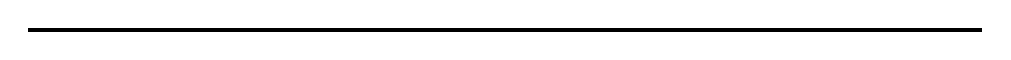
\begin{tikzpicture}
        	\draw[line cap=rect, color=leftsideaccent, line width=1.5pt] (0,0) -- (\textwidth-1.5pt,0);
    	\end{tikzpicture}

		\vspace{\leftsidetextpadding}

		%%%%%%%%%%%%%%%%%%%%%%%%%%%%%
		%     	  QUALITIES     	%
		%%%%%%%%%%%%%%%%%%%%%%%%%%%%%

		% <qualities>
		% <contents>
		% <quality section>
		% <section name>
		{\large \fontfamily{qbk}\selectfont \color{leftsideaccent} \textbf{%
			Qualitiy Section% section name
		}}

		\begin{flushleft}
			\renewcommand{\arraystretch}{1.1}
			\begin{tabular}{ll}
		% </section name>
		% <items>
		% <level>
				\progressbar{4em}{%
				0.9% level
		}%
		% </level>
		% <quality>
		&%
				Comp 1% quality
		% </quality>
		\\
		% </items>
			\end{tabular}
		\end{flushleft}

		\bigskip

		% </quality section>
		% </contents>
		% </qualities>

    \end{minipage}%
    }%
    \end{center}%
\end{minipage}%
}%
\colorbox{debugyellow}{%
\begin{minipage}[\textheight]{\textwidth-\leftsideratio\textwidth}%
    \begin{center}%
    \vspace{\margins}%
    \colorbox{debuggreen}{%
    \color{rightsidetext}
    %%%%%%%%%%%%%%%%%%%%%%%%%%%%%%%%%%%%%%%%%%%%%%%%%%%%%%%%%
    %                                                       %
    %                      RIGHT SIDE                       %
    %                                                       %
    %%%%%%%%%%%%%%%%%%%%%%%%%%%%%%%%%%%%%%%%%%%%%%%%%%%%%%%%%
    \begin{minipage}[t][\textheight-\margins]{0.9\textwidth}%
    	\vspace{\margins}%
   		%%%%%%%%%%%%%%%%%%%%%%%%%%%%%%%%%%%%%%%%%%%%%%%%%%%%%%%%%
   	 	%                HEADLINE & ABOUT ME                    %
    	%%%%%%%%%%%%%%%%%%%%%%%%%%%%%%%%%%%%%%%%%%%%%%%%%%%%%%%%%
    	\begin{flushleft}%
    		{\Huge \color{rightsideaccent} \fontfamily{qbk}\selectfont \textbf{\name}}
    	\end{flushleft}

    	\ifthenelse{\not\equal{\aboutme}{}}{%

    	\bigskip

    	\textit{\aboutme}
    	}{}

		\bigskip

    	\vspace{\rightsidetextpadding}

    	%%%%%%%%%%%%%%%%%%%%%%
		%     	VITA		     %
		%%%%%%%%%%%%%%%%%%%%%%

        % <vita>
		% <vita section>
		% <title>
    	{\LARGE \color{rightsideaccent} \fontfamily{qbk}\selectfont \textbf{%
    		Experience% title
    	}}

    	\bigskip

    	% </title>
		% <contents>
		% <vita item>

		\CVItem{%
		% <title>
			Job Title% title
		% </title>
		}{%
		% <start date>
			from% start date
		% </start date>
		}{%
		% <end date>
			to% end date
		% </end date>
		}{%
		% <organisation>
			Company% organisation
		% </organisation>
		}

		% <description>

		\begin{itemize}[topsep=2pt, partopsep=0pt, parsep=0pt, itemsep=0pt]
		% <description items>
		% <item>
 			\item%
 			item1% item
 		% </item>
		% </description items>
 		\end{itemize}

		% </description>

		\bigskip

		% </vita item>
		% </contents>

    	\vspace{\rightsidetextpadding}

		% </vita section>
		% </vita>

    \end{minipage}
    }
    \end{center}
\end{minipage}
}

\end{document}
